\documentclass[12pt]{article}
\usepackage[margin=2.5cm]{geometry}
\usepackage{enumerate}
\usepackage{amsfonts}
\usepackage{amsmath}
\usepackage{fancyhdr}
\usepackage{amsmath}
\usepackage{amssymb}
\usepackage{amsthm}
\usepackage{mdframed}
\usepackage{graphicx}
\usepackage{subcaption}
\usepackage{adjustbox}
\usepackage{listings}
\usepackage{xcolor}
\usepackage{booktabs}
\usepackage[utf]{kotex}

\definecolor{codegreen}{rgb}{0,0.6,0}
\definecolor{codegray}{rgb}{0.5,0.5,0.5}
\definecolor{codepurple}{rgb}{0.58,0,0.82}
\definecolor{backcolour}{rgb}{0.95,0.95,0.92}

\lstdefinestyle{mystyle}{
    backgroundcolor=\color{backcolour},
    commentstyle=\color{codegreen},
    keywordstyle=\color{magenta},
    numberstyle=\tiny\color{codegray},
    stringstyle=\color{codepurple},
    basicstyle=\ttfamily\footnotesize,
    breakatwhitespace=false,
    breaklines=true,
    captionpos=b,
    keepspaces=true,
    numbers=left,
    numbersep=5pt,
    showspaces=false,
    showstringspaces=false,
    showtabs=false,
    tabsize=1
}

\lstset{style=mystyle}

\begin{document}
\title{CSC236 Worksheet 3}
\author{Hyungmo Gu}
\maketitle

\section*{Question 1}

\bigskip

\begin{itemize}
    \item
    Given the statement to prove

    \bigskip

    \begin{center}
        $P(x,y,z):$ There are no positive integers $x,y,z$ such that $x^3 + 3y^3 = 9z^3$
    \end{center}

    \bigskip

    \begin{proof}

        We will prove $P(x,y,z)$ using proof by contradiction.

        \bigskip

        Assume $\exists x,y,z \in \mathbb{N}^{+}$, $x^3 + 3y^3 = 9z^3$.

        \bigskip

        First, we need to show there is smallest element $x_0 \in X$ with $y_0,z_0 \in \mathbb{N}^+$
        satisfying $x^3 + 3y^3 = 9z^3$, using well-ordering principle.

        \bigskip

        The header tells us there are elements $x,y,z \in \mathbb{N}^+$, satisfying
        $x^3 + 3y^3 = 9z^3$.

        \bigskip

        Then, we can write the set $X = \{x \mid x \in \mathbb{N}^+,\:\exists y,z \in
        \mathbb{N}^+,\:x^3 + 3y^3 = 9z^3\}$ is not empty.

        \bigskip

        Then, using principle of well-ordering, we can write that there is smallest
        positive natural number $x_0 \in X$ along with $y_0,z_0 \in \mathbb{N}^+$ satisfying
        $x^3 + 3y^3 = 9z^3$.

        \bigskip

        Second, we need to show that $x_1^3 = 9z_1^3 - 3y_1^3$ is satisfied, given
        $x_0 > x_1$.

        \bigskip

        We will do so in parts.

        \bigskip

        \underline{\textbf{Part 1 (Showing $x_0 = 3 \cdot x_1$):}}

        \bigskip

        We know that

        \begin{align}
            x_0^3 + 3y_0^3 &= 9z_0^3\\
            x_0^3 &= 9z_0^3 - 3y_0^3
        \end{align}

        \bigskip

        Since $3 \mid 9z_0^3 - 3y_0^3$, we can write $3 \mid x_0^3$.

        \bigskip

        Then, since 3 is a prime number, by using the hint provided in question 3
        of assignment 1, we can write there is $x_1 \in \mathbb{Z}$, $x_0 = 3 \cdot x_1$.

        \bigskip

        Then, because we know $x_0, 3 \in \mathbb{N}^+$, we can conclude
        $x_1 \in \mathbb{N}^+$.

        \bigskip

        \underline{\textbf{Part 2 (Showing $y_0 = 3 \cdot y_1$):}}

        \bigskip

        We know that

        \begin{align}
            x_0^3 + 3y_0^3 &= 9z_0^3\\
            3y_0^3 &= 9z_0^3 - x_0^3
        \end{align}

        \bigskip

        Then, using the fact $x_0 = 3 \cdot x_1$ from part 1, we can calculate

        \begin{align}
            3y_0^3 &= 9z_0^3 - 3^3x_1^3\\
            y_0^3 &= 3z_0^3 - 3^2x_1^3
        \end{align}

        \bigskip

        Since $3 \mid 3z_0^3 - 3^2x_1^3$, we can write that $3 \mid y_0^3$.

        \bigskip

        Then, since 3 is a prime number, by using the hint provided in question 3
        of assignment 1, we can write there is $y_1 \in \mathbb{Z}$, $y_0 = 3 \cdot y_1$.

        \bigskip

        Then, because we know $y_0, 3 \in \mathbb{N}^+$, we can conclude
        $y_1 \in \mathbb{N}^+$.

        \bigskip

        \underline{\textbf{Part 3 (Showing $z_0 = 3 \cdot z_1$):}}

        \bigskip

        We know that

        \begin{align}
            9z_0^3 &= x_0^3 + 3y_0^3
        \end{align}

        \bigskip

        Then, using the fact $x_0 = 3 \cdot x_1$ from part 1, and
        $y_0 = 3 \cdot y_1$ from part 2, we can calculate

        \begin{align}
            9z_0^3 &= 3^3x_1^3 + 3^4y_1^3\\
            z_0^3 &= 3x_1^3 + 3^2y_1^3
        \end{align}

        \bigskip

        Since $3 \mid 3x_1^3 + 3^2y_1^3$, we can write that $3 \mid z_0^3$.

        \bigskip

        Then, since 3 is a prime number, by using the hint provided in question 3
        of assignment 1, we can write there is $z_1 \in \mathbb{Z}$, $z_0 = 3 \cdot z_1$.

        \bigskip

        Then, because we know $z_0, 3 \in \mathbb{N}^+$, we can conclude
        $z_1 \in \mathbb{N}^+$.

        \bigskip

        \underline{\textbf{Part 4 (Showing $x_1^3 = 9z_1^3 - 3y_1^3$):}}

        \bigskip

        We know that

        \begin{align}
            9z_0^3 &= x_0^3 + 3y_0^3
        \end{align}

        \bigskip

        Then, using the fact $x_0 = 3 \cdot x_1$ from part 1,
        $y_0 = 3 \cdot y_1$ from part 2, and $z_0 = 3 \cdot z_1$ we can calculate

        \begin{align}
            3^5z_1^3 &= 3^3x_1^3 + 3^4y_1^3\\
            3^2z_1^3 &= x_1^3 + 3y_1^3\\
            9z_1^3 &= x_1^3 + 3y_1^3
        \end{align}

        \bigskip

        Finally, the part 4 tells us

        \begin{align}
            9z_1^3 &= x_1^3 + 3y_1^3
        \end{align}

        where $x_1 < x_0$.

        \bigskip

        Then, because we know $x_0$ is the smallest
        number satisfying $x^3 + 3y^3 = 9z^3$, we can conclude above leads to
        contradiction.

        \bigskip

        Then, we can conclude the the assumption is false.

    \end{proof}
\end{itemize}

\bigskip

\underline{\textbf{Notes:}}

\begin{itemize}
    \item \underline{\textbf{Proof By Contradiction:}} $\neg P \Rightarrow \neg Q \land Q$ (Assuming
    we are proving $P \Rightarrow Q$)
    \item \underline{\textbf{Principle of Well-Ordering:}} Any nonempty subset $A$
    of $\mathbb{N}$ contains a minimum element; i.e. for any $A \subseteq \mathbb{N}$
    such that $A \neq \emptyset$, there is some $a \in A$ such that for all $a' \in A$, $a \leq a'$.

    \item examples of well-ordered sets
    \begin{enumerate}[1.]
        \item $\mathbb{N} \cup \{0\}$
        \item $\mathbb{N} \cup \{1,2\}$
        \item $\{n \in \mathbb{N}: n > 5\}$
    \end{enumerate}
    \item examples of non-well-ordered sets
    \begin{enumerate}[1.]
        \item $\mathbb{R}$ and the open interval $(0,2)$
        \item $\mathbb{Z}$
    \end{enumerate}

    \item Learned the $P$ in $\neg P \Rightarrow \neg Q \land Q$ is the statement

    \bigskip

    \begin{center}
        $P(x,y,z):$ There are no positive integers $x,y,z$ such that $x^3 + 3y^3 = 9z^3$
    \end{center}

    \bigskip

    And learned the $Q$ is the principle of well-ordering on $P$.

    \item Learned the goal of contradiction is to show the assumption violates principle
    of well-ordering. That is, there is $x_1 \in X$ less than $x_0$ satisfying
    $x^3 + 3y^3 = 9z^3$

    \item Noticed professor reduced wordiness of work using short notations.

    \begin{center}
    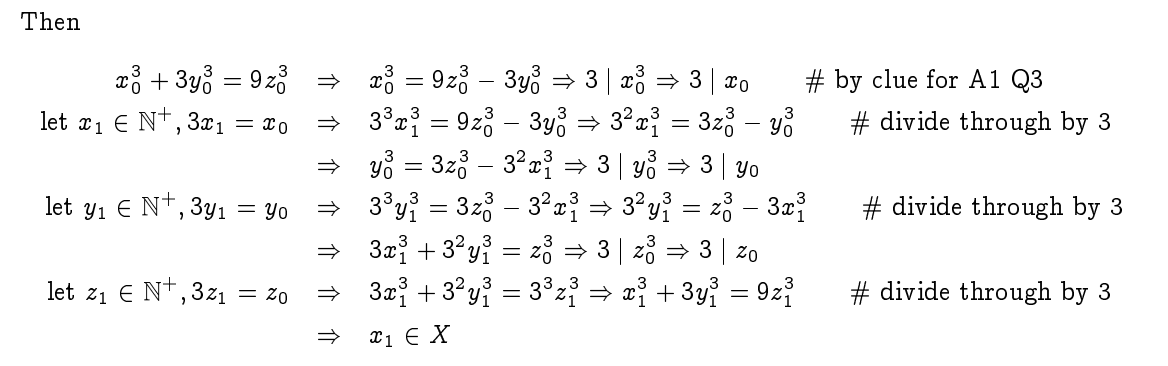
\includegraphics[width=0.8\linewidth]{images/worksheet_3_q1_note.png}
    \end{center}

\end{itemize}


% \begin{mdframed}
%     \underline{\textbf{Rough Work:}}

%     \bigskip

%     \textbf{Predicate Logic:} $\forall A \subseteq \mathbb{N},\:A \neq \emptyset \Rightarrow
%     (\exists a \in A, \: \forall x \in A,\: a \leq x)$

%     \bigskip

%     Given the statement to prove

%     \bigskip

%     \begin{center}
%         $P(x,y,z):$ There are no positive integers $x,y,z$ such that $x^3 + 3y^3 = 9z^3$
%     \end{center}

%     \bigskip

%     We will prove $P(x,y,z)$ using proof by contradiction.

%     \bigskip

%     Assume $\exists x,y,z \in \mathbb{N}^{+}$, $x^3 + 3y^3 = 9z^3$.

%     \begin{enumerate}[1.]

%         \item State that there is smallest element $x_0 \in X$ with $y_0,z_0 \in \mathbb{N}^+$
%         satisfying $x^3 + 3y^3 = 9z^3$, using well-ordering principle

%         \bigskip

%         First, we need to show there is smallest element $x_0 \in X$ with $y_0,z_0 \in \mathbb{N}^+$
%         satisfying $x^3 + 3y^3 = 9z^3$, using well-ordering principle.

%         \bigskip

%         \begin{mdframed}
%         First, we need to show there is smallest element $x_0 \in X$ with $y_0,z_0 \in \mathbb{N}^+$
%         satisfying $x^3 + 3y^3 = 9z^3$, using well-ordering principle.

%         \bigskip

%         The header tells us there are elements $x,y,z \in \mathbb{N}^+$, satisfying
%         $x^3 + 3y^3 = 9z^3$.

%         \bigskip

%         Then, we can write the set $X = \{x \mid x \in \mathbb{N}^+,\:\exists y,z \in
%         \mathbb{N}^+,\:x^3 + 3y^3 = 9z^3\}$ is not empty.

%         \bigskip

%         Then, using principle of well-ordering, we can write that there is smallest
%         positive natural number $x_0 \in X$ along with $y_0,z_0 \in \mathbb{N}^+$ satisfying
%         $x^3 + 3y^3 = 9z^3$.
%         \end{mdframed}

%         \item Show that $x_1^3 = 9z_1^3 - 3y_1^3$ is satisfied, given $x_0 > x_1$

%         \bigskip

%         Second, we need to show $x_1^3 = 9z_1^3 - 3y_1^3$ is satisfied, given
%         $x_0 > x_1$.

%         \bigskip

%         We will do so in parts.

%         \bigskip

%         \begin{itemize}
%             \item First, show that $x_0 = 3 \cdot x_1$, using $x_0^3 + 3y_0^3 = 9z_0^3$ and the
%             fact if a prime number $p$ divides a perfect cube $n^3$, then $p$ also divides $n$.

%             \begin{mdframed}
%             \underline{\textbf{Part 1 (Showing $x_0 = 3 \cdot x_1$):}}

%             \bigskip

%             We know that

%             \begin{align}
%                 x_0^3 + 3y_0^3 &= 9z_0^3\\
%                 x_0^3 &= 9z_0^3 - 3y_0^3
%             \end{align}

%             \bigskip

%             Since $3 \mid 9z_0^3 - 3y_0^3$, we can write $3 \mid x_0^3$.

%             \bigskip

%             Then, since 3 is a prime number, by using the hint provided in question 3
%             of assignment 1, we can write there is $x_1 \in \mathbb{Z}$, $x_0 = 3 \cdot x_1$.

%             \bigskip

%             Then, because we know $x_0, 3 \in \mathbb{N}^+$, we can conclude
%             $x_1 \in \mathbb{N}^+$.

%             \end{mdframed}

%             \item Second, show that $y_0 = 3 \cdot y_1$, using $x_0^3 = 3^3 x_1^3 = 9z_0^3 - 3y_0^3$

%             \begin{mdframed}
%             \underline{\textbf{Part 2 (Showing $y_0 = 3 \cdot y_1$):}}

%             \bigskip

%             We know that

%             \begin{align}
%                 x_0^3 + 3y_0^3 &= 9z_0^3\\
%                 3y_0^3 &= 9z_0^3 - x_0^3
%             \end{align}

%             \bigskip

%             Then, using the fact $x_0 = 3 \cdot x_1$ from part 1, we can calculate

%             \begin{align}
%                 3y_0^3 &= 9z_0^3 - 3^3x_1^3\\
%                 y_0^3 &= 3z_0^3 - 3^2x_1^3
%             \end{align}

%             \bigskip

%             Since $3 \mid 3z_0^3 - 3^2x_1^3$, we can write that $3 \mid y_0^3$.

%             \bigskip

%             Then, since 3 is a prime number, by using the hint provided in question 3
%             of assignment 1, we can write there is $y_1 \in \mathbb{Z}$, $y_0 = 3 \cdot y_1$.

%             \bigskip

%             Then, because we know $y_0, 3 \in \mathbb{N}^+$, we can conclude
%             $y_1 \in \mathbb{N}^+$.

%             \end{mdframed}

%             \item Third, show that $z_0 = 3 \cdot z_1$, using $x_0^3 = 3^3 x_1^3 = 9z_0^3 - 3y_0^3 =  9z_0^3 - 3^4y_1^3$

%             \begin{mdframed}
%             \underline{\textbf{Part 3 (Showing $z_0 = 3 \cdot z_1$):}}

%             \bigskip

%             We know that

%             \begin{align}
%                 9z_0^3 &= x_0^3 + 3y_0^3
%             \end{align}

%             \bigskip

%             Then, using the fact $x_0 = 3 \cdot x_1$ from part 1, and
%             $y_0 = 3 \cdot y_1$ from part 2, we can calculate

%             \begin{align}
%                 9z_0^3 &= 3^3x_1^3 + 3^4y_1^3\\
%                 z_0^3 &= 3x_1^3 + 3^2y_1^3
%             \end{align}

%             \bigskip

%             Since $3 \mid 3x_1^3 + 3^2y_1^3$, we can write that $3 \mid z_0^3$.

%             \bigskip

%             Then, since 3 is a prime number, by using the hint provided in question 3
%             of assignment 1, we can write there is $z_1 \in \mathbb{Z}$, $z_0 = 3 \cdot z_1$.

%             \bigskip

%             Then, because we know $z_0, 3 \in \mathbb{N}^+$, we can conclude
%             $z_1 \in \mathbb{N}^+$.

%             \end{mdframed}

%             \item Finally, show $x_1^3 = 9z_1^3 - 3y_1^3$

%             \begin{mdframed}
%             \underline{\textbf{Part 4 (Showing $x_1^3 = 9z_1^3 - 3y_1^3$):}}

%             \bigskip

%             We know that

%             \begin{align}
%                 9z_0^3 &= x_0^3 + 3y_0^3
%             \end{align}

%             \bigskip

%             Then, using the fact $x_0 = 3 \cdot x_1$ from part 1,
%             $y_0 = 3 \cdot y_1$ from part 2, and $z_0 = 3 \cdot z_1$ we can calculate

%             \begin{align}
%                 3^5z_1^3 &= 3^3x_1^3 + 3^4y_1^3\\
%                 3^2z_1^3 &= x_1^3 + 3y_1^3
%             \end{align}

%             \end{mdframed}
%         \end{itemize}

%         \bigskip

%         \begin{mdframed}
%         Second, we need to show that $x_1^3 = 9z_1^3 - 3y_1^3$ is satisfied, given
%         $x_0 > x_1$.

%         \bigskip

%         We will do so in parts.

%         \bigskip

%         \underline{\textbf{Part 1 (Showing $x_0 = 3 \cdot x_1$):}}

%         \bigskip

%         We know that

%         \begin{align}
%             x_0^3 + 3y_0^3 &= 9z_0^3\\
%             x_0^3 &= 9z_0^3 - 3y_0^3
%         \end{align}

%         \bigskip

%         Since $3 \mid 9z_0^3 - 3y_0^3$, we can write $3 \mid x_0^3$.

%         \bigskip

%         Then, since 3 is a prime number, by using the hint provided in question 3
%         of assignment 1, we can write there is $x_1 \in \mathbb{Z}$, $x_0 = 3 \cdot x_1$.

%         \bigskip

%         Then, because we know $x_0, 3 \in \mathbb{N}^+$, we can conclude
%         $x_1 \in \mathbb{N}^+$.

%         \bigskip

%         \underline{\textbf{Part 2 (Showing $y_0 = 3 \cdot y_1$):}}

%         \bigskip

%         We know that

%         \begin{align}
%             x_0^3 + 3y_0^3 &= 9z_0^3\\
%             3y_0^3 &= 9z_0^3 - x_0^3
%         \end{align}

%         \bigskip

%         Then, using the fact $x_0 = 3 \cdot x_1$ from part 1, we can calculate

%         \begin{align}
%             3y_0^3 &= 9z_0^3 - 3^3x_1^3\\
%             y_0^3 &= 3z_0^3 - 3^2x_1^3
%         \end{align}

%         \bigskip

%         Since $3 \mid 3z_0^3 - 3^2x_1^3$, we can write that $3 \mid y_0^3$.

%         \bigskip

%         Then, since 3 is a prime number, by using the hint provided in question 3
%         of assignment 1, we can write there is $y_1 \in \mathbb{Z}$, $y_0 = 3 \cdot y_1$.

%         \bigskip

%         Then, because we know $y_0, 3 \in \mathbb{N}^+$, we can conclude
%         $y_1 \in \mathbb{N}^+$.

%         \bigskip

%         \underline{\textbf{Part 3 (Showing $z_0 = 3 \cdot z_1$):}}

%         \bigskip

%         We know that

%         \begin{align}
%             9z_0^3 &= x_0^3 + 3y_0^3
%         \end{align}

%         \bigskip

%         Then, using the fact $x_0 = 3 \cdot x_1$ from part 1, and
%         $y_0 = 3 \cdot y_1$ from part 2, we can calculate

%         \begin{align}
%             9z_0^3 &= 3^3x_1^3 + 3^4y_1^3\\
%             z_0^3 &= 3x_1^3 + 3^2y_1^3
%         \end{align}

%         \bigskip

%         Since $3 \mid 3x_1^3 + 3^2y_1^3$, we can write that $3 \mid z_0^3$.

%         \bigskip

%         Then, since 3 is a prime number, by using the hint provided in question 3
%         of assignment 1, we can write there is $z_1 \in \mathbb{Z}$, $z_0 = 3 \cdot z_1$.

%         \bigskip

%         Then, because we know $z_0, 3 \in \mathbb{N}^+$, we can conclude
%         $z_1 \in \mathbb{N}^+$.

%         \bigskip

%         \underline{\textbf{Part 4 (Showing $x_1^3 = 9z_1^3 - 3y_1^3$):}}

%         \bigskip

%         We know that

%         \begin{align}
%             9z_0^3 &= x_0^3 + 3y_0^3
%         \end{align}

%         \bigskip

%         Then, using the fact $x_0 = 3 \cdot x_1$ from part 1,
%         $y_0 = 3 \cdot y_1$ from part 2, and $z_0 = 3 \cdot z_1$ we can calculate

%         \begin{align}
%             3^5z_1^3 &= 3^3x_1^3 + 3^4y_1^3\\
%             3^2z_1^3 &= x_1^3 + 3y_1^3\\
%             9z_1^3 &= x_1^3 + 3y_1^3
%         \end{align}

%         \end{mdframed}

%         \item Conclude that this contracts the original claim that $x_0$ is the smallest
%         non-negative value satisfying $x^3 + 3y^3 = 9z^3$.

%         \begin{mdframed}
%         Finally, the part 4 tells us

%         \begin{align}
%             9z_1^3 &= x_1^3 + 3y_1^3
%         \end{align}

%         where $x_1 < x_0$.

%         \bigskip

%         Then, because we know $x_0$ is the smallest
%         number satisfying $x^3 + 3y^3 = 9z^3$, we can conclude above leads to
%         contradiction.

%         \bigskip

%         Then, we can conclude the the assumption is false.
%         \end{mdframed}
%     \end{enumerate}

% \end{mdframed}

\section*{Question 2}

\bigskip

\begin{mdframed}
    \underline{\textbf{Rough Work:}}

    \bigskip

    \begin{enumerate}[1.]
        \item Basis

        \begin{mdframed}
        \underline{\textbf{Basis:}}

        \bigskip

        We need to show that the property is true for the simplest members $x,y,z$.

        \bigskip

        There are three cases: $e = x$, $e = y$ and $e = z$. In each of the cases
        $s_2(e) = 1$ and $s_1(e) = 0$.

        \bigskip

        Using this fact, starting from the left hand side, we can conclude
        \setcounter{equation}{0}
        \begin{align}
            s_1(e) = 0 &= 3 \cdot 0\\
            &= 3 \cdot (1 - 1)\\
            &= 3 \cdot (s_2(e) - 1)
        \end{align}
        \end{mdframed}

        \item Inductive Step

        \bigskip

        Let $e_1$ and $e_2$ be arbitrary elements of $\varepsilon$.
        Assume $H({e_1,e_2}):$ $P(e_1)$ and $P(e_2)$. That is, $e_1$ and $e_2$
        have the property $s_1(e_1) = 3 \cdot (s_2(e) - 1)$ and
        $s_1(e_2) = 3 \cdot (s_2(e_2) - 1)$.

        \bigskip

        We need to show all possible combinations of $e_1$ and $e_2$ have the
        property. That is, $P((e_1 + e_2))$, $P((e_1 \times e_2))$.

        \bigskip

        \begin{mdframed}
        \underline{\textbf{Inductive Step:}}

        \bigskip
        Let $e_1$ and $e_2$ be arbitrary elements of $\varepsilon$.
        Assume $H({e_1,e_2}):$ $P(e_1)$ and $P(e_2)$. That is, $e_1$ and $e_2$
        have the property $s_1(e_1) = 3 \cdot (s_2(e) - 1)$ and
        $s_1(e_2) = 3 \cdot (s_2(e_2) - 1)$.

        \bigskip

        We need to show all possible combinations of $e_1$ and $e_2$ have the
        property. That is, $P((e_1 + e_2))$, $P((e_1 \times e_2))$.

        \bigskip

        There are two cases, depending on how $e$ is constructed from $e_1$ and $e_2$:
        $e = (e_1 + e_2)$, $e = (e_1 \times e_2)$.
        In each case we have

        \begin{align}
            s_1(e) = s_1(e_1) + s_1(e_2) + 3 & \\
            s_2(e) = s_2(e_2) + s_2(e_2)
        \end{align}

        \bigskip

        Then, using above fact, we can conclude

        \bigskip

        \begin{align}
            s_1(e) &= s_1(e_1) + s_1(e_2) + 3 & [\text{by 4}]\\
            &= 3 \cdot (s_2(e_1) - 1) + 3 \cdot (s_2(e_2) - 1) + 3 & [\text{by induction hypothesis}]\\
            &= 3 \cdot s_2(e_1) - 3 + 3 \cdot s_2(e_2) - 3 + 3\\
            &= 3 \cdot s_2(e_1) + 3 \cdot s_2(e_2) - 6 + 3\\
            &= 3 \cdot ( s_2(e_1) + s_2(e_2)) - 3\\
            &= 3 \cdot s_2(e) - 3 & [\text{by 5}]
        \end{align}

        \end{mdframed}

        \begin{mdframed}

        \end{mdframed}
    \end{enumerate}
\end{mdframed}

\bigskip

\underline{\textbf{Notes:}}

\bigskip

\begin{itemize}
    \item \textbf{Structural Induction}
    \begin{itemize}
        \item is a proof method used in mathematical logic, computer science, graph theory.
        \item is a generalization of mathematical induction over natural numbers.
        \item is a recursion method
        \item
        \underline{\textbf{Example:}}

        \begin{mdframed}

            Define $\varepsilon$: The smallest set such that
            \begin{itemize}
                \item $x,y,z \in \varepsilon$ \color{red}\# variables\color{black}
                \item $e_1, e_2 \in \varepsilon \Rightarrow (e_1 + e_2), (e_1 - e_2),
                (e_1 \times e_2),(e_1 \div e_2) \in \varepsilon$ \color{red}\# operators\color{black}
            \end{itemize}

            \bigskip

            (steps omitted). Prove $P(e):\:\textbf{vr}(e) = \textbf{op}(e) + 1$ \color{red}\# \textbf{vr} means number of variable,
            \textbf{op} means number of operators\color{black}

        \end{mdframed}

        \bigskip

        to prove above using structural induction:

        \bigskip

        \begin{enumerate}[1.]
            \item \textbf{Verify Base Case(s):} Show that the property is true for the
            simplest members, {x,y,z}. That is show $P(x)$, $P(y)$, and $P(z)$.

            \begin{mdframed}
            There are three cases: $e =x$, $e = y$, and $e = z$. In each case $\textbf{vr}(e) = 1$
            and $\textbf{op}(e) = 0$, so $P(e)$ holds for the basis.
            \end{mdframed}

            \item \textbf{Inductive Step:} Let $e_1$ and $e_2$ be arbitrary elements of $\varepsilon$.
            Assume $H({e_1,e_2}):$ $P(e_1)$ and $P(e_2)$. That is, $e_1$ and $e_2$
            have the property $\textbf{vr}(e_1) = \textbf{op}(e_1) + 1$ and
            $\textbf{vr}(e_2) = \textbf{op}(e_2) + 1$.

            \bigskip

            We need to show all possible combinations of $e_1$ and $e_2$ have the
            property. That is, $P((e_1 + e_2))$, $P((e_1 - e_2))$, $P((e_1 \times e_2))$,
            and $P((e_1 \div e_2))$.

            \begin{mdframed}

            There are four cases, depending on how $e$ is constructed from $e_1$ and $e_2$:
            $e = (e_1 + e_2)$, $e = (e_1 - e_2)$, $e = (e_1 \times e_2)$ and $e = (e_1 \div e_2)$.
            In each case we have

            \begin{align}
                \textbf{vr}(e) = \textbf{vr}(e_1) + \textbf{vr}(e_2) & \\
                \textbf{op}(e) = \textbf{op}(e_1) + \textbf{op}(e_2) + 1 & \color{red}\text{\# +1 is from + in $e_1 + e_2$}
            \end{align}

            \bigskip

            Thus,

            \begin{align}
                \textbf{vr}(e) &= \textbf{vr}(e_1) + \textbf{vr}(e_2) & [\text{by (4.1)}]\\
                &= (\textbf{op}(e_1) + 1) + (\textbf{op}(e_2) + 1) & [\text{by induction hypothesis}]\\
                &= (\textbf{op}(e_1) + \textbf{op}(e_2)) + 2\\
                &= (\textbf{op}(e) - 1) + 2 & [\text{by (4.2)}]\\
                &= \textbf{op}(e) + 1
            \end{align}

            \end{mdframed}
        \end{enumerate}
    \end{itemize}
\end{itemize}

\section*{Question 3}

\end{document}